%=======================02-713 LaTeX template, following the 15-210 template==================
%
% You don't need to use LaTeX or this template, but you must turn your homework in as
% a typeset PDF somehow.
%
% How to use:
%    1. Update your information in section "A" below
%    2. Write your answers in section "B" below. Precede answers for all 
%       parts of a question with the command "\question{n}{desc}" where n is
%       the question number and "desc" is a short, one-line description of 
%       the problem. There is no need to restate the problem.
%    3. If a question has multiple parts, precede the answer to part x with the
%       command "\part{x}".
%    4. If a problem asks you to design an algorithm, use the commands
%       \algorithm, \correctness, \runtime to precede your discussion of the 
%       description of the algorithm, its correctness, and its running time, respectively.
%    5. You can include graphics by using the command \includegraphics{FILENAME}
%
\documentclass[11pt]{article}
\usepackage{amsmath,amssymb,amsthm}
\usepackage{graphicx}
\usepackage[margin=1in]{geometry}
\usepackage{fancyhdr}
\setlength{\parindent}{0pt}
\setlength{\parskip}{5pt plus 1pt}
\setlength{\headheight}{13.6pt}
\newcommand\question[2]{\vspace{.25in}\hrule\textbf{#1: #2}\vspace{.5em}\hrule\vspace{.10in}}
\renewcommand\part[1]{\vspace{.10in}\textbf{(#1)}}
\newcommand\algorithm{\vspace{.10in}\textbf{Algorithm: }}
\newcommand\correctness{\vspace{.10in}\textbf{Correctness: }}
\newcommand\runtime{\vspace{.10in}\textbf{Running time: }}
\pagestyle{fancyplain}
\lhead{\textbf{\NAME\ (\ANDREWID)}}
\chead{\textbf{Assignment \HWNUM - PolInt}}
\rhead{\today}

\usepackage{IEEEtrantools}
\usepackage{listings}
\usepackage{caption}
\usepackage{subcaption}
\usepackage{subfig}
\usepackage{wrapfig,lipsum,booktabs}

% Python style for highlighting
\newcommand\pythonstyle{\lstset{
language=Python,
basicstyle=\ttm,
otherkeywords={self},             % Add keywords here
keywordstyle=\ttb\color{deepblue},
emph={MyClass,__init__},          % Custom highlighting
emphstyle=\ttb\color{deepred},    % Custom highlighting style
stringstyle=\color{deepgreen},
frame=tb,                         % Any extra options here
showstringspaces=false            % 
}}


% Python environment
\lstnewenvironment{python}[1][]
{
\pythonstyle
\lstset{#1}
}
{}

\begin{document}\raggedright
%Section A==============Change the values below to match your information==================
\newcommand\NAME{Surajkumar H}  % your name
\newcommand\ANDREWID{EE11B075}     % your andrew id
\newcommand\HWNUM{1}              % the homework number
%Section B==============Put your answers to the questions below here=======================

% no need to restate the problem --- the graders know which problem is which,
% but replacing "The First Problem" with a short phrase will help you remember
% which problem this is when you read over your homeworks to study.

\question{1}{Question 1: 5-point 4th order Interpolation} 
\setcounter{section}{1}
%\part{a} \algorithm Describe algorithm here

In this question, we sample the function $f(x)=sin(x+x^2)$ uniformly at 5 points in $[0,1]$. We then use these 5 sample values to interpolate (and extrapolate) the function values at points in the range given by 
\begin{lstlisting}
xx=np.linspace(0,1,5);
\end{lstlisting}

\subsection{Background and Functions}

We examine how polynomial interpolation performs at these values and compare it with the theoretical (known) value of the function at these points. Since we have exactly 5 samples, we run $4^{th}$ order polynomial interpolation on all points in the range. We use the modified Neville's Algorithm. The original algorithm constructs the Lagrangian polynomial recursively, running interpolation on smaller sets (of say $m$) points, and uses adjacent sets to estimate the value of the interpolation using $m+1$ points. The recursive relation is
\begin{equation}
P_{i(i+1)\ldots(i+m)} = \frac{(x-x_{i+m})P_{i(i+1)\ldots(i+m-1)}+(x_{i}-x)P_{(i+1)(i+2)\ldots(i+m)}}{x_i - x_{i+m}}
\end{equation}

where $x$ is the point where the function value is to be inter(extra)polated. By design, the function values coincide with the data values at the known sample points.  

The modified version of the algorithm (which we use here) starts with an initial estimate of the function value (we do this by finding the sample closest to the point of interest), and recursively computing \textit{small differences} between adjacent estimates (using the smaller sets as above). We choose one of these differences at each stage, and add it to the function estimate at the point of interest. Mathematically, we define for $m=1,2,\ldots,N-1$
\begin{IEEEeqnarray}{rCl}
C_{m,i} &=& P_{i(i+1)\ldots(i+m)} - P_{i(i+1)\ldots(i+m-1)} \nonumber \\
D_{m,i} &=& P_{i(i+1)\ldots(i+m)} - P_{(i+1)(i+2)\ldots(i+m)}
\end{IEEEeqnarray}
that is, the upper and lower differences in the ancestor tree (as seen in \cite{NR}). From this, we get

\begin{IEEEeqnarray}{rCl}
C_{m+1,i} &=& \frac{(x_{i+m+1}-x)(C_{m,i+1}-D_{m,i})}{x_{i}-x_{i+m+1}} \nonumber \\
D_{m+1,i} &=& \frac{(x_{i}-x)(C_{m,i+1}-D_{m,i})}{x_{i}-x_{i+m+1}} \label{nev1}
\end{IEEEeqnarray}

At each level $m$, the $Cs$ and $Ds$ represent the corrections made to the value estimate. We recursively compute these corrections using \ref{nev1}. We then choose a path through the ancestor tree which connects the final interpolated value ($m=N-1$), to the initial estimate. We then add all these corrections to get the interpolated value at the point $x$. In our implementation of the algorithm, we chose the correction based on whether the index estimate is above / below the average ($\frac{N-m}{2}$). This way, we ensure  movement towards the rightmost element correctly. 

A general python function \textsc{polint} was written (based on the code in \cite{NR}), which computes the $N^{th}$ order interpolated value at a single point from the set of data points and values. The function \textsc{findnearest} takes an input point, the entire data set, the order of interpolation $N$, and computes indices of the nearest $N$ data points. Later, we test how the error varies with the order of interpolation. It is very helpful to have a function which finds the closes $N$ samples for a given value, since we can use these to interpolate the function value at the unknown point $x$. Finally, we used $\textsc{nearestpolint}$ to perform point by point inter(extra)polation on every point in $xx$ (set of unknown values). 

\begin{figure*}
        \centering
        \begin{subfigure}{.5\textwidth}
  \centering
        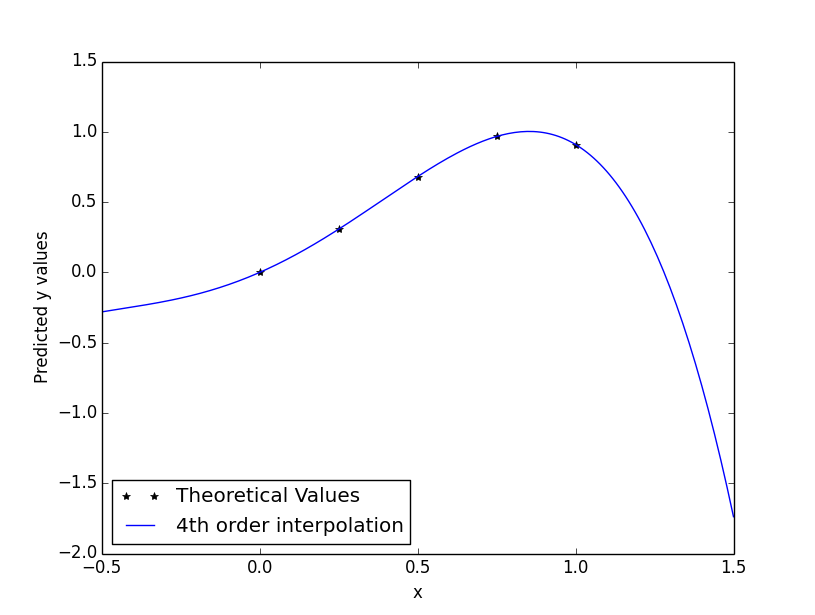
\includegraphics[width=\linewidth]{q1/interpol.png}
                \caption{Theoretical and interpolated values of $f(x)$}
                \label{fig:q1_inter}
                \end{subfigure}%
\begin{subfigure}{.5\textwidth}
  \centering
        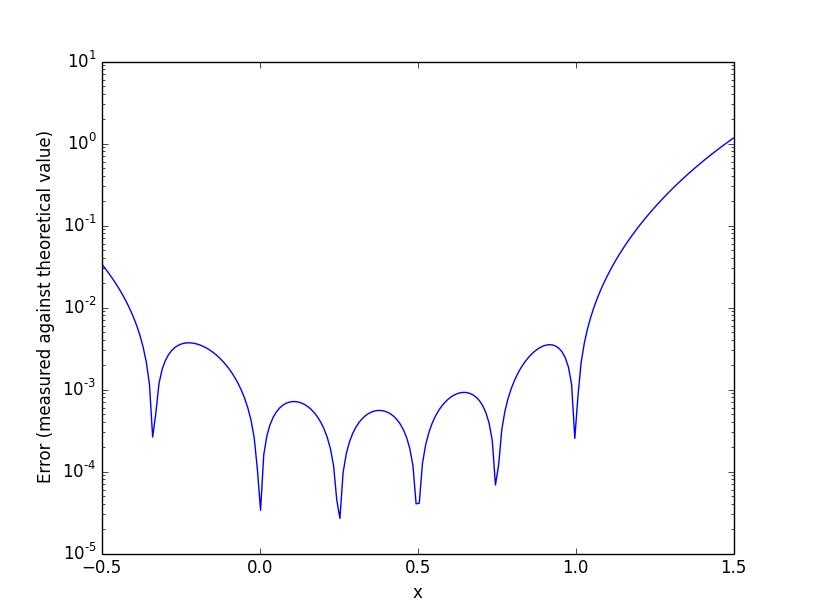
\includegraphics[width=\linewidth]{q1/error_log.png}
                \caption{$4^{th}$ order Interpolation error}
                \label{fig:q1_error}
	\end{subfigure}
            
\caption{Comparison of theoretical and $4^{th}$-order inter(extra)polated function values, and the absolute error in interpolation}
\label{fig:q1}            
\end{figure*}

\subsection{Interpolation, Extrapolation and Error}
\label{exp1}

Figure (\ref{fig:q1_inter}) shows the comparison of the theoretical, and the 4th order interpolated value at the intermediate and outer points. Figure (\ref{fig:q1_error}) shows the error in 4th order interpolation, taken with respect to the theoretical function values at the point (given by $f(x)$). We clearly see that the error at the interpolated points is of the order $10^{-3}$ for middle points, and $~10^{-2}$ as we move closer to the edge. This makes sense, as the data at the edge doesn't give us equal information on how the function behaves on both sides (which middling values give us). The spike values indicate the known points, where the error is $0$ (the log should be $-\infty$, but python ignores the value), and the points very close to the known point have a smaller error. As we go closer to the midpoint between any 2 known values, the error increases. 

The behaviour beyond $[0,1)$ is a lot more unpredictable. For this particular function, the error increases as we move further away from the known points. We are using $N^{th}$ order (N=4) interpolation. We are trying to fit an $Nth$ order polynomial to a given set of $N$ points. The function $f(x)$ is a sine, and thus has an infinite Taylor expansion. The smallest error that could creep in depends on the derivative of the function near the known points, and how far the function is from the nearest sample points ($\Delta x^{N})$). The further away we go, the higher the error. 
As we can clearly see, the polynomial fit $\to\pm\infty$ as $x\to\pm\infty$. This means as we go further away from the known data points, the extrapolated function blows up. Since the actual $f(x)$ is bounded (maximum value is $1$), the error value grows larger with $x$ (cannot guarantee monotonicity). 

\pagebreak 
 
\question{2}{Question 2: 30-point 4th order Interpolation} 
\setcounter{section}{2}

\begin{figure*}
        \centering
        \begin{subfigure}{.5\textwidth}
  \centering
        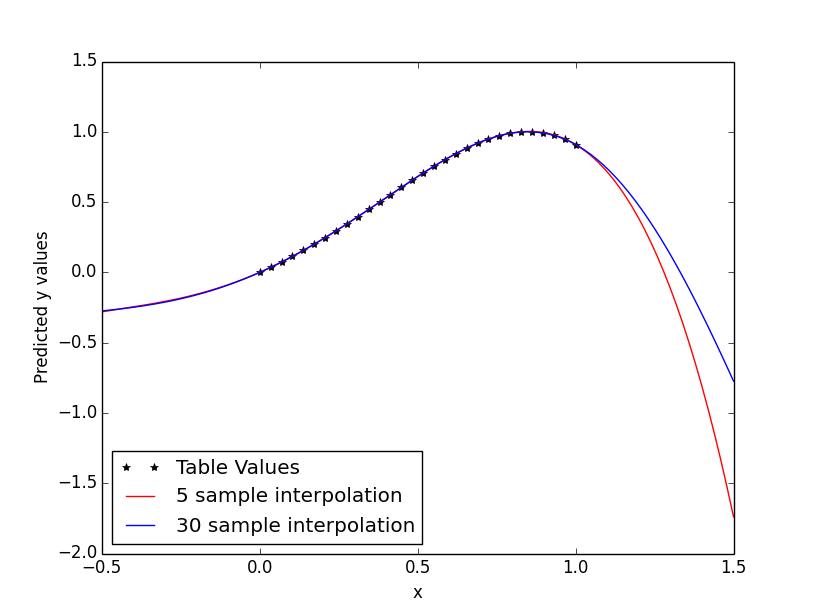
\includegraphics[width=\linewidth]{q2/interpol.png}
                \caption{Theoretical and interpolated values of $f(x)$}
                \label{fig:q2_inter}
                \end{subfigure}%
\begin{subfigure}{.5\textwidth}
  \centering
        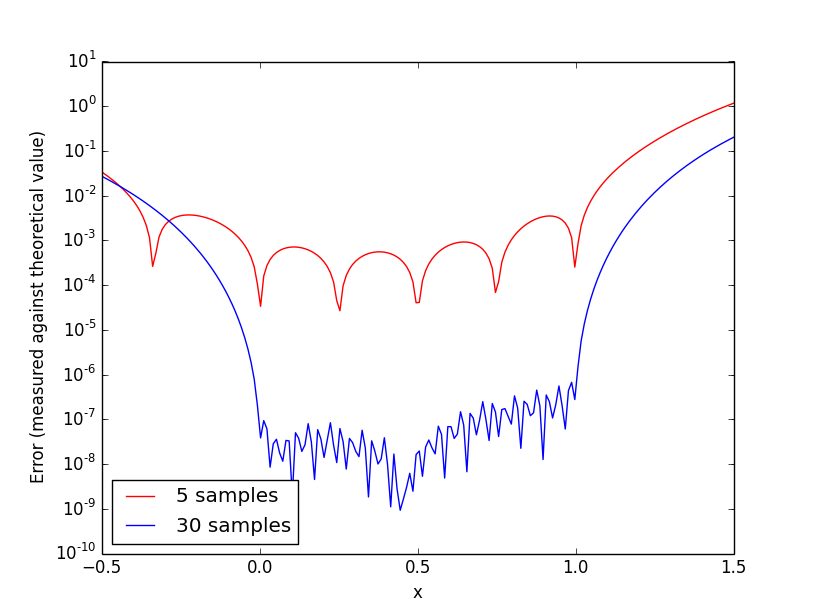
\includegraphics[width=\linewidth]{q2/error_log.png}
                \caption{Comparison of $4^{th}$ order Interpolation error run for 5 and 30 sample points}
                \label{fig:q2_error}
	\end{subfigure}
            
\caption{Comparison of theoretical and $4^{th}$-order inter(extra)polated function values obtained using 5 and 30 sample points}
\label{fig:q2}            
\end{figure*}

In this problem, we investigate the effect of higher sample point density on interpolation. Specifically, we compare the previous case of $4th$ order interpolation with 5 sample points, to $4th$ order interpolation with 30 sample points. We use \textsc{findnearest} to find the nearest 5 points for any given point, and then use \textsc{polint} to find the interpolated value. We run this over the same data set as in the first question. 

Intuitively, we expect denser interpolation to give much lower error. This is because we fit the same order polynomial over a much closer set of points. Since the function is 'nice' (the function doesn't have discontinuous derivatives), the local behaviour of the function described by 5 close sample points should give a closer approximation of the function, as compared to 5 far away points. This makes sense, as the closer the points, the slower the change in higher-order derivatives (since the function is 'nice'), and the less the cost involved in ignoring the higher order derivatives (they change less rapidly over the interval as we decrease the sample spacing). So the function is better approximated by a given order of interpolation with closer data points.

Figure (\ref{fig:q2_inter}) shows the comparison of the theoretical, the 5 sample and the 30 sample interpolation. Figure (\ref{fig:q2_error}) shows the absolute error comparison for the 2 cases. The plot agrees with our intuition. The interpolation error is roughly $~10^{-3}$ for the 5 sample version, and $~10^{-7}$ for the 30 sample version.

It is not easy to make a statement about extrapolation in this setting. Comparing the 2 different sampling frequency cases is not trivial, as the sharper/flatter slope given to us by the denser samples may/may not be the better approximation to the function behaviour at far away points. We can make a general statement that extrapolation will have a much higher error as compared to interpolation. Using the same argument as in Section \ref{exp1}, the error increases (not necessarily monotonic) as we go further away from the known samples. 
%We can't really give a concrete general statement on how the sample density affects the extrapolation error, ans it affects the nature of the function at the point of interest, and at the nearest samples. 

\question{3}{Question 3: Order of Interpolation and Error} 
\setcounter{section}{3}

\begin{figure*}
        \centering
        \begin{subfigure}{.5\textwidth}
  \centering
        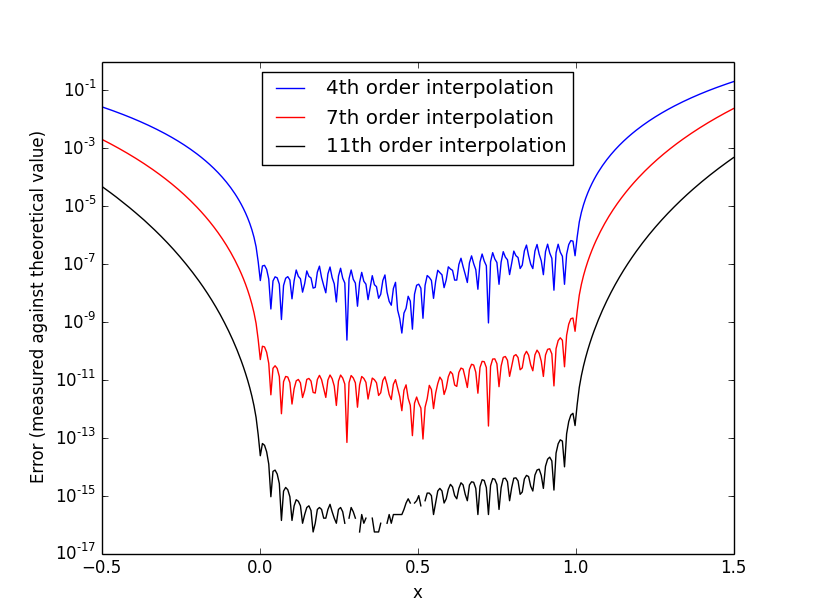
\includegraphics[width=\linewidth]{q3/error_comp.png}
                \caption{Error in various interpolation schemes close the known points}
                \label{fig:q3_close}
                \end{subfigure}%
\begin{subfigure}{.5\textwidth}
  \centering
        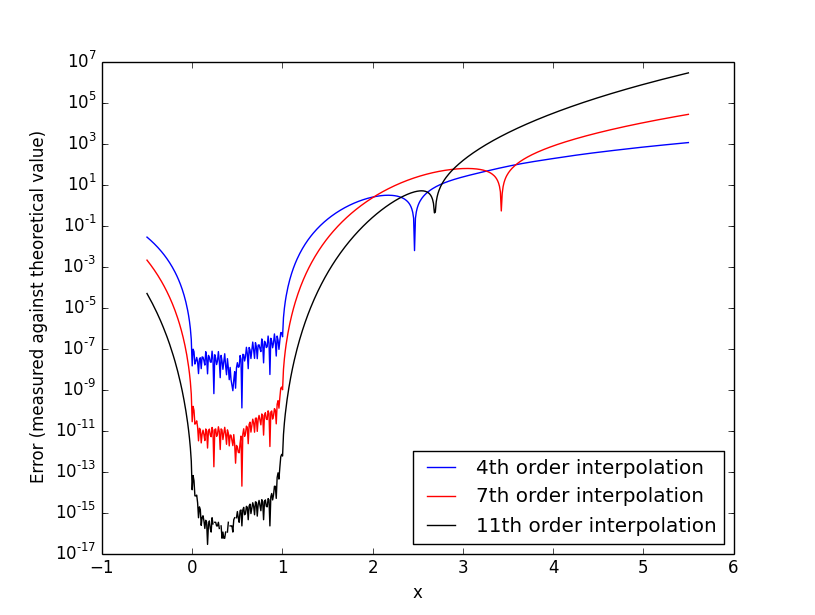
\includegraphics[width=\linewidth]{q3/error_far.png}
                \caption{Extrapolation error given by polynomial interpolation at far away points}
                \label{fig:q3_far}
	\end{subfigure}
            
\caption{Absolute errors introduced by $4^{th}$-order,$7^{th}$-order and $11^{th}$-order interpolation obtained using 30 sample points in $[0,1)$}
\label{fig:q3}            
\end{figure*}

Here, we investigate the effect of changing the degree of the interpolation used in out \textsc{PolInt} function. Recall that in $N^{th}$-order polynomial interpolation, we are essentially fitting a polynomial of order $N-1$ through the $N$ given data points. 

As we increase the order of interpolation, we are allowing more sample points to become a part of the decision for a given point. We are also allowing for the flexibility in the interpolating polynomial, allowing it to exhibit more accurate behaviour. This combination of more information and more flexibility intuitively tells us that increasing the order of interpolation might lower the error (not guaranteed, as other errors can creep in). 

Mathematically, for any given point, the function is described by its complete Taylor series. At best, an interpolating polynomial of order $N-1$ can match the first $N$ terms of the Taylor series. The lower bound on error is $\frac{f^{(N)}(\zeta)}{N!}\Delta x^{N}$ ($\zeta$ is a point anywhere in the range bounded by the sample points). For sample points fairly close together ($\Delta x<1$), the upper bound on error $\Omega(\Delta x^{N})$ decreases as $N$ increases. The error is allowed to (but not guaranteed) to reduce this way.

Figure (\ref{fig:q3_close}) shows the behaviour near the interpolated points. We see a reduction in the error magnitudes as the order of interpolation increases. We also notice some flat-ish regions in the $11th$-order interpolation curve, as the errors get $~10^{-17}$. We conjecture that the error is due to python's inability to represent the number, rather than a shortcoming of the interpolation algorithm. 

Figure (\ref{fig:q3_far}) shows the extrapolation error, and how it varies with order of interpolation. We see that the extrapolation error increases with $x$ (not monotonically). We notice from the graph that the extrapolation error is higher at far away points (for sufficiently large $x$). 

\pagebreak

\begin{figure*}
        \centering
        \begin{subfigure}{.5\textwidth}
  \centering
        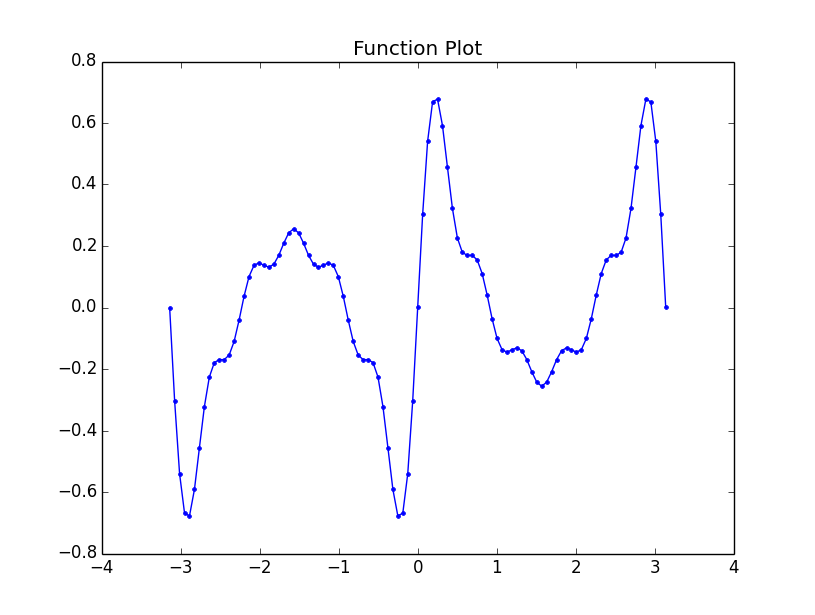
\includegraphics[width=\linewidth]{q4/function.png}
                \caption{Function plot for a 5 term truncated Fourier series}
                \label{fig:q4_5}
                \end{subfigure}%
\begin{subfigure}{.5\textwidth}
  \centering
        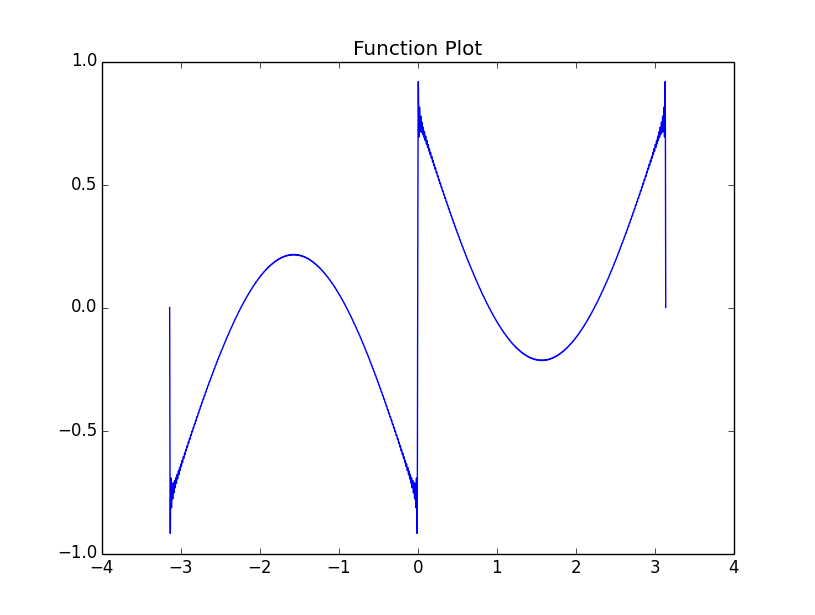
\includegraphics[width=\linewidth]{q4/function_200.png}
                \caption{Function plot for a 200 term truncated Fourier series}
                \label{fig:q4_200}
	\end{subfigure}
            
\caption{Function plots for truncated fourier series}
\label{fig:q4}            
\end{figure*}

\question{4}{Question 4: Truncated Fourier Series}

In this question, we analyse the truncated Fourier Series given by 
\begin{equation}
f(x) = \sum_{k=1}^5 \frac{sin(2k+1)x}{2k+1}
\end{equation}
For the numerical parts of the question, we sample $f(x)$ uniformly at 101 points in $[-\pi,\pi]$. The first part of the question is about the full series, given by $g(x)=\sum_{k=1}^{\infty} \frac{sin(2k+1)x}{2k+1}$. Consider the behaviour of the function about $x=0$. At $x=0$, the function value is $g(0)=0$. At $x=0^{+}$, all the sines take positive values. So, we can upper-bound it as $g(0^+) \leq \sum_{k=1}^{\infty} \frac{1}{2k+1} = \infty$, as $\sum_k \frac{1}{k}$ is a divergent series. 

Similarly, at $x=0^{-}$, the sines all take negaative values. So, $g(0^-) \geq \sum_{k=1}^{\infty} \frac{-1}{2k+1} = -\infty$. 

It is difficult to find the exact behaviour of the function near zero, so we turned to python. Taking $200$ terms of the series instead of 5 showed us that $g(0^+)\approx 1$ and $g(0^-)\approx -1$. So the series is discontinuous at $x=0$. The same argument holds at all $x=\pm n\pi$, so the function itself has many discontinuities. 

Since the full series itself is discontinuous at $x=\pm n\pi$, all its derivatives are discontinuous (they take infinite values at some points) at $x=\pm n\pi$. 

In contrast, the truncated series is just the sum of a finite number of sines, and so is continuous. By linearity of differentiation, the truncated series will be analytic (infinitely differentiable) everywhere. 
    
\pagebreak
    
    
\question{5}{Question 5: Periodic Functions, Interpolation and Error}

\begin{figure*}
        \centering
        \begin{subfigure}{.5\textwidth}
  \centering
        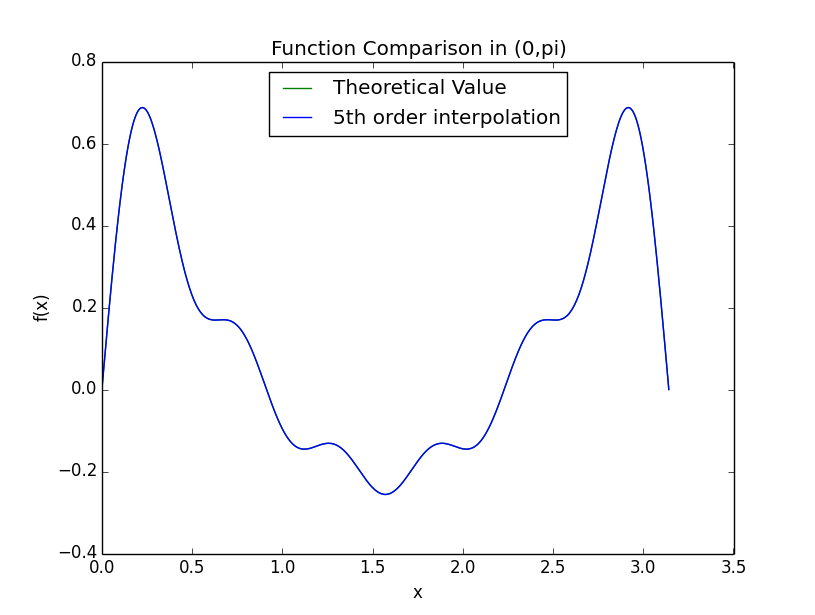
\includegraphics[width=\linewidth]{q5/interpol.png}
                \caption{Function plot in $[0,\pi]$}
                \label{fig:q5_interpol}
                \end{subfigure}%
\begin{subfigure}{.5\textwidth}
  \centering
        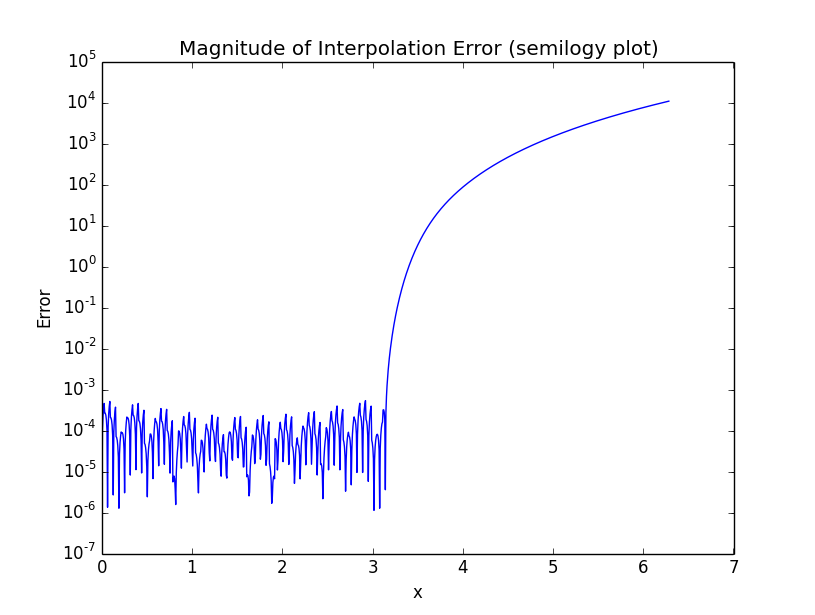
\includegraphics[width=\linewidth]{q5/error.png}
                \caption{Absolute inter(extra)polation error}
                \label{fig:q5_error}
	\end{subfigure}
            
\caption{5th order polynomial interpolation on the Truncated Fourier series}
\label{fig:q5}            
\end{figure*}

In this part, we perform $5^{th}$ oreder interpolation to find the function behaviour in the range $[0,2\pi]$. Since the truncated series is smooth, the logic and the inferences we draw are quite similar to the previous questions. \

For the points in $[0,\pi]$, there are nearby known sample values. Since the  point density is very high, the error is quite low. Figure (\ref{fig:q5_interpol}) shows us how well the function mirrors the theoretical value in this range. 

Outside this range, the error increases rapidly (using the arguments for question 3). The function itself is periodic, and should be bounded. The nearest points after $\pi$ cause the interpolated value to drop steeply, thus causing a very high error value. The error increases as we move further away from the known point, and hits $10^{3}$ error and higher very quickly. 

The behaviour at $-\pi,\pi$ is as expected from the 5-term truncated series. Since we are using polynomial interpolation, the values at these 2 points will be exactly the same as the theoretical value (these were sample points). Since the truncated series itself is smooth, the error doesn't exhibit an order-of-magnitude change at the end points (as compared to the middle). It behaves very much like how we would expect normal polynomial interpolation to behave.

If we go closer to the full series, the situation becomes very different. Take for example the 200-term truncated series as in Figure (\ref{fig:q4_200}). The derivative values near $x=\pm n\pi$ are very high, and the function undergoes a sharp change. Polynomial interpolation will find it harder to model such a sharp change, and so the error will be much higher near $x=\pm n\pi$

If we assume the user tells us the function is periodic, we can greatly improve our estimate by sampling and interpolating within a period, and simply repeating our interpolated values after every period. If the user gives us the time period after which the function repeats, it is trivial. 

On the other hand, if the user just gives us a table of function values, and guarantees periodicity inside this set of values, we can find the period. The brute force way is to take the first point, and scan through the rest of the table to find all occurrences of the same point. Say it occurs at indices ${u_1,u_2,\ldots u_j}$ We then take the second point, and compare the function value with the values at ${u_1+1,u_2+1,\ldots u_j+1}$. We find all the points where the values are identical. Repeat or the 3rd, 4th and so on until we hit $u_1$. The smallest index gives us the number of samples in a period. The number of comparisons needed here depends on the function period quite heavily.

Another way is to compute the derivatives at each point (using function differences) upto say the $Mth$ derivative (M=5 say). At every period, the samples behave identically, and so the derivatives will be identical. We can take the first point, and scan through the table until we find a point whose derivatives line up exactly with the derivatives of the first point. This gives us the sample period. Unlike in the previous scheme, we do an order-sense fixed number of computations (independent of period). Taking too small a value of $M$ could cause us to assume a smaller time period, which could lead to error by itself, so the $M$ needs to be chosen carefully. 

\question{6}{Question 6: Maximal Extrapolation Error}

\begin{wraptable}{r}{6.5cm}
\caption{Maximum Error values for various interpolation orders}
\renewcommand{\arraystretch}{1.0}
\label{tab:1}
\begin{tabular}{c|c} \toprule
PolInt Order & Maximum Error \\\midrule
3 & 9.79693175e+01 \\  
4 & 8.77092699e+02 \\  
5 & 1.07820283e+04 \\  
6 & 9.42259464e+03 \\  
7 & 3.42607319e+05 \\  
8 & 1.54103744e+06 \\  
9 & 2.57607062e+06 \\  
10 & 3.71325255e+07 \\  
11 & 6.48419631e+07 \\  
12 & 3.40994870e+08 \\  
13 & 1.62883681e+09 \\  
14 & 1.57671653e+08 \\  
15 & 1.51654626e+10 \\  
16 & 3.29396712e+10 \\  
17 & 5.27810681e+10 \\  
18 & 3.33898559e+11 \\  
19 & 2.58667561e+11 \\  
20 & 1.56763845e+12 \\  \bottomrule
\end{tabular}
\end{wraptable} 


For this question, we find the maximum inter(extra)polation error in this range. From a numerical perspective, all we had to do was loop over many interpolation orders for the sample points in this range, find the largest error for each order, and compare the various orders. We compare interpolation orders ranging from $3-20$. 

As we pointed out for the earlier questions, we see a general upward trend in the maximum extrapolation error. The lower bound on error scales as $\Omega(\Delta x^{N})$ for $(N-1)th$ order interpolation. So for far away points, increasing $N$ increases the lower bound on error. The actual values of maximum error depend on many other factors, such as the behaviour of the function near the end-points. For the given function and set of data points, $20^{th}$-order polynomial interpolation seems to yield the highest error.

There are certain values where the maximum extrapolation error decreases for a higher order, but increases afterword. The scale of errors like these are also very high. We get nearly $10^{8}$ error with certain types of interpolation. This motivates the need for finding and periodically repeating interpolated values, especially if we know the function is periodic. 
    
\vspace{1.0em}    
    
\question{7}{Non-Analytic functions and Interpolation}    
\setcounter{section}{7}  
\setcounter{subsection}{0}

This problem involves finding a 6-digit accurate method to calculate

\begin{equation}
f(x) = \frac{sin(\pi x)}{\sqrt{1-x^2}}
\end{equation}
    
\subsection{Analyticity and Radius of Convergence}
    
The function takes 0 value at $x=0$. At $x=1$, L'Hospital rule tells us that the function takes value 0. The first derivative is given by
\begin{equation}
f'(x) = \frac{\pi \sqrt{1-x^2}cos(\pi x) - \frac{x}{\sqrt{1-x^2}} sin(\pi x)}{1-x^2}
\end{equation}
Based on this, $f'(1)=-\infty$ (verifiable numerically). From the function graph (Figure (\ref{fig:q7_interpol})), we see that the slope near $x=1$ is $\infty$. So the first derivative is discontinuous at $x=1$. Whatever the order of differentiation, the singularities introduced will only by at $x=\pm 1$. At all other points, it is a combination of analytic functions, and so, is analytic in $[0,1)$. The Radius of convergence (RoC) of the function is $[0,1)$. As we approach $x=1$, the function approaches a steady value, but the rate of approach is extremely high. This sharp increase in the first derivative will affect polynomial interpolation, which might  struggle to fit a fast-changing enough curve to the given function. 

 

\subsection{Achieving 6-digit accuracy}

We see from the above analysis that the function changes rapidly near $x=1$. So we expect that a given order of polynomial interpolation should give higher errors as compared to lower $x$. This makes sense, as we are trying to fit an $Nth$ order polynomial to something that changes a lot faster than a polynomial. . Increasing the order of the polynomial should allow us to model a higher rate of change, and thus give a lower probability of error.

Figure (\ref{fig:q7_err6}) shows 5th order interpolation, where for the most part, the error is low, but increases as we get closer to $x=1$. The peak error in this case is $~10^{-4}$. 

\begin{figure*}[h]
        \centering
        \begin{subfigure}{.5\textwidth}
  \centering
        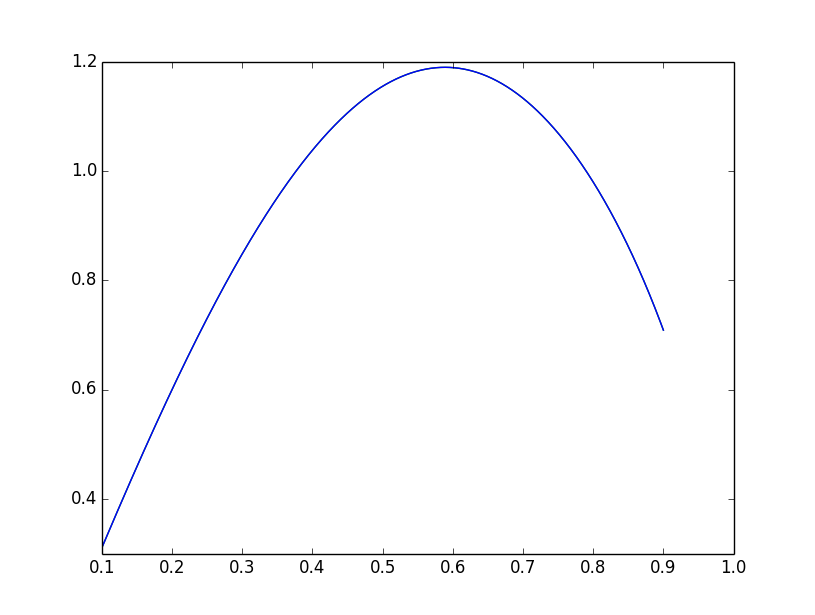
\includegraphics[width=\linewidth]{q7/interpol.png}
                \caption{Function plot in $[0,0.991]$}
                \label{fig:q7_interpol}
                \end{subfigure}%
\begin{subfigure}{.5\textwidth}
  \centering
        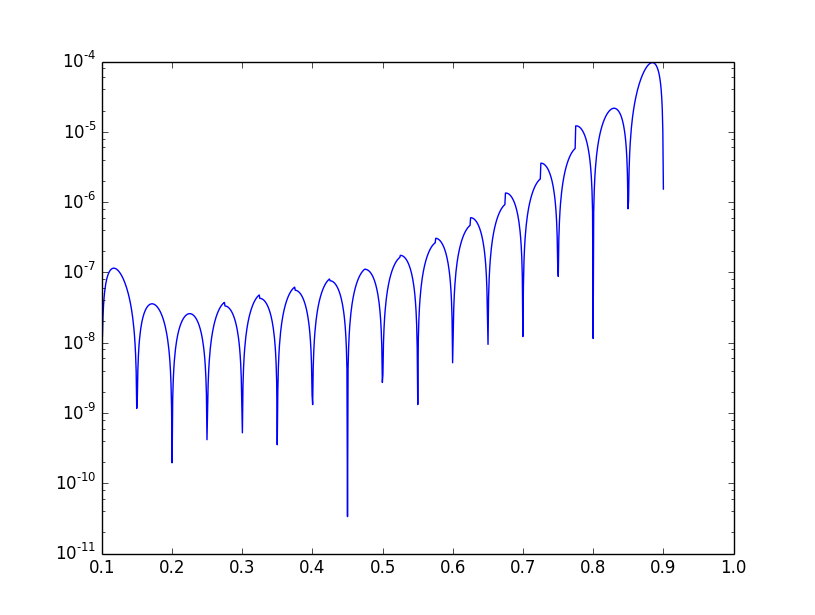
\includegraphics[width=\linewidth]{q7/err_6.png}
                \caption{5th order interpolation with sample spacing 0.05}
                \label{fig:q7_err6}
	\end{subfigure}
	\caption{Function plot for $f(x)$ and a first-attempt at }
\end{figure*}           
        
         \pagebreak
  \begin{figure*}
        \centering
        \begin{subfigure}{.5\textwidth}
  \centering
        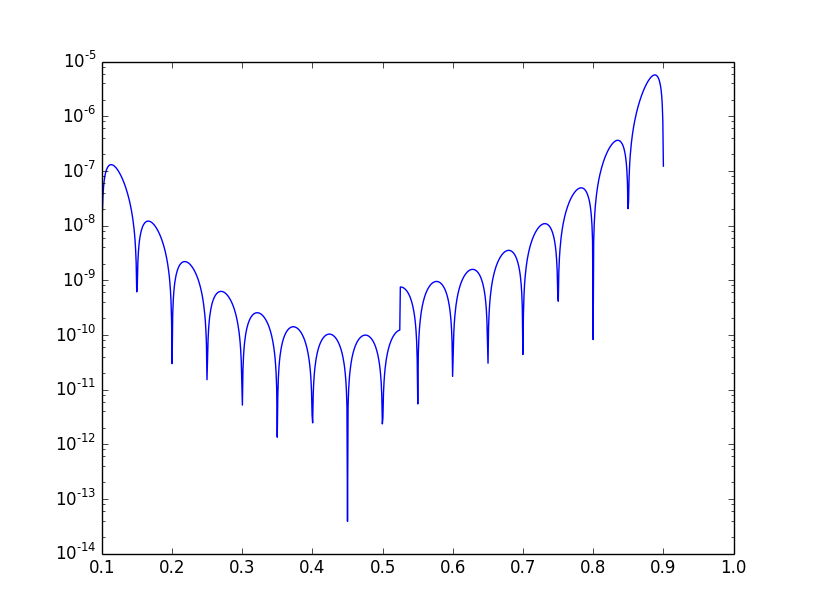
\includegraphics[width=\linewidth]{q7/err_16.png}
                \caption{15th order interpolation with sample spacing 0.05}
                \label{fig:q7_err16}
                \end{subfigure}%
\begin{subfigure}{.5\textwidth}
  \centering
        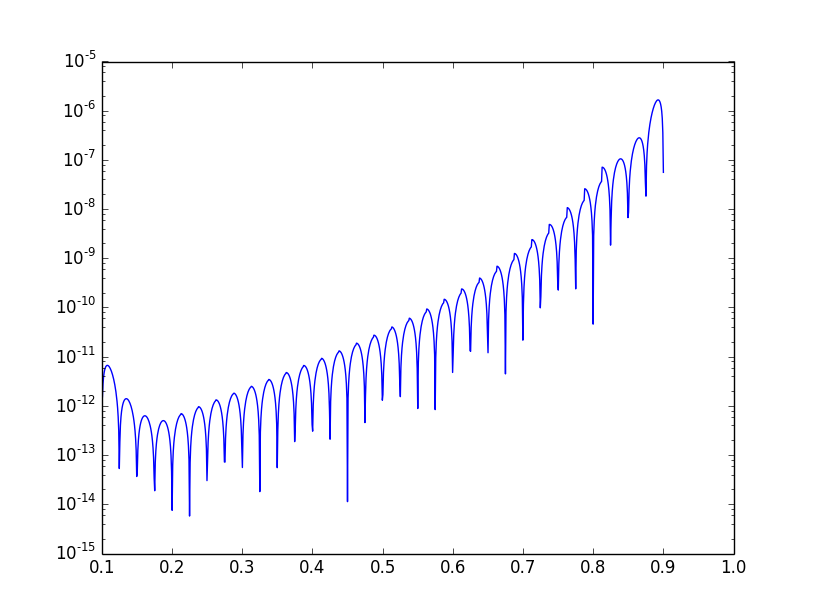
\includegraphics[width=\linewidth]{q7/err_over.png}
                \caption{6th order interpolation with sample spacing 0.025}
                \label{fig:q7_err_over}
	\end{subfigure}
            
\caption{Two different ways of achieving 6-digit accuracy, use a very high order interpolation, or reduce the sample spacing.}
\label{fig:q7}            
\end{figure*}

The first method of achieving 6-digit accuracy is by increasing the interpolation order, while maintaining the sample spacing. 
This is shown in Figure (\ref{fig:q7_err16}), where we use 15th-order interpolation. Even this gives us at-best an error of $~10^{-5}$, while we need $~10^{-7}$ to ensure 6-digit accuracy.

Motivated by Question 3, we try to improve accuracy by increasing the sample density. We do this by reducing the sample spacing (to 0.02 from 0.05). Figure (\ref{fig:q7_err_over}) shows the error plot for 6th-order interpolation with 0.02 sample spacing. The error probability is much lower at lower $x$, but increases more steeply. Choosing a reasonable order of interpolation, or very small sample spacing gives us the required accuracy. 

This question shows us that polynomial interpolation becomes less accurate as we approach the non-analytic points. We can increase the order of interpolation, or reduce the sample spacing to reduce the peak error. 
\begin{thebibliography}{155}
\bibitem{NR}
William H. Press, Saul A. Teukolsky, William T. Vetterling, Brian P. Flannery, "Numerical Recipes in C" 

\bibitem{Stoer}
J. Stoer, R. Bulirsch, "Introduction to Numerical Analysis"

\end{thebibliography}


\end{document}
